\chapter{Implementation Tree Edit Distance}
In this chapter we present the implementation of Shasha and Zhangs algorithm by Henderson~\cite{Hen}. We discuss meaningful choices of cost functions and compare them with each other. We present a short overview over our solutions which then leads us to our next chapter where we compare the experiences of Shasha and Zhang's algorithm and the GRF.

\section{Shasha and Zhang's algorithm by Henderson}
Suppose we want to compute the tree edit distance for two trees $A$ and $B$. Henderson's implementation can be split into two separated important steps:
\begin{enumerate}
\item Finding out the post-order traversal index and the keyroots for the two trees under consideration.
\item Computing the tree edit distances for all relevant subproblems, i.e. combinations of subtrees induced by keyroots of $A$ and $B$ respectively.
\end{enumerate}

\underline{Ad Step $1$}:\\
In Listing~\ref{lst:AnnTree} we present the initialization of the class AnnotatedTree. It can be split up into two parts: Step $1$a) and Step $1$b). We will give a short summary of what happens in these two substeps later on.
\lstinputlisting[language=Python, caption=Initialization of an AnnotatedTree, label=lst:AnnTree]{figures/annotated_tree.py}
\underline{Ad Step $1$a)}:\\
This substep initializes a stack $pstack$ that is needed for the Step $1$b). But first we take a close look at the variable called $stack$. A stack is a specific data structure. It is a collection of objects that supports fast last-in, first-out semantics. Throughout the process of the loop, the stack always consists of a pair of data, namely a node and a list of all its ancestors. Therefore we initialize the stack with the pair of the annotated tree's root and an empty collection, since the root doesn't have an ancestor. \\
While the stack still contains some pair of data we perform a function on it called \textit{pop}. This function returns the last element of the stack and removes it from the stack. We associate every node with a unique id $nid$. If the inspected node has some children we enlarge the stack with pairs of each children and the updated list of ancestors. The essential detail is that we \textit{append} this pair to the stack, which means that we put it on the end of the stack. The reason why this is so important will be explained later. After appending all children to the stack, the node will be appended to another stack called $pstack$ which will be used in Step $1$b), together with its node id $nid$ and the list of ancestors.
Let's go through the process for the first pair of data, namely the root and the empty set of ancestors. We assign the $nid$ $0$ to the root and go through its children. Here we first append the root's left child, afterwards its right child. Thus the right child is further in the back of the stack than the left child. Since we only $pop$ the stack, the right child will be out of the stack earlier than the left child. Furthermore, during the next loop we append the stack with other nodes again, pushing the left child of the root further down the stack. Thus we end up with the new stack $pstack$ that has the correct left to right post traversal ordering. The further back a node is in the stack $pstack$, the smaller is its post traversal ordering index.
\\
\underline{Ad Step $1$b)}:\\
In this step we determine the keyroots of the investigated tree. The key idea is, that a node is a keyroot if and only if it is the node with the highest post-order traversal index among all nodes with the same left most descendant. The right sibling of a node $n$ has a different left most descendant than the node $n$ itself. But any node with a higher index can not have the same left most descandant as this right sibling because of the way we indexed the nodes. Thus if we determine the node with the highest index among all nodes that share the same leftmost descendant, then we know that it has to be a keyroot. For this we need two temporary dictionaries $lmds$, the list of the left most descendant for every node, and $keyroots$, a dictionary that saves the highest index of all nodes that share a leftmost descendant.\\
As previously discussed we go through $pstack$, a stack of nodes in the correct order. The counter $i$ saves the actual post order index, it increments after every loop. 
During every loop we pop the stack and get a node $n$, its node id $nid$ and its ancestors. Then we check whether the node is a leaf or not. If it indeed is, then we set the left most descendant of every ancestor to this node, as long as it does not already have a left most descendant. If it is an interior node, then we just get the left most descendant by checking the dictionary $lmds$. The most important step happens near the end of the loop: setting $keyroots[lmd] = i$. In this way we find the highest index $i$ of all nodes, that share the same leftmost descendant. Therefore, after having finished the routine, we get the keyroots by checking the values of the temporary dictionary $keyroots$.

This was a detailed description of the way an object of type AnnotatedTree gets initialized. It makes use of efficiently appending and popping a stack to receive the correct indexing and the all the necessary information to get the list of keyroots.

\underline{Ad Step $2$}:\\
After the initialization of the AnnotatedTree, the actual computation of the tree edit distance is done by first considering all relevant subproblems. A distance matrix is created that stores the pairwise distance between all relevant subproblems of the two investigated trees. This matrix gets built incrementally by applying the recursion stated in Lemma~\ref{lem:saz}. The technical details can be seen in the actual implementation~\cite{Hen}.

\section{Distance measures}
The most simple distance measure for the tree edit distance just counts the number of operations needed to transform one tree into the other. This implies that any insertion, any deletion and any renaming costs the same value of $1$. We call this distance measure the \textit{standard tree edit distance} (STED)\\
The big difference between the tree edit distance and the gRF is that the latter does not take the interior nodes of the trees into account, structural differences like inserting an interior node to prolong the path at some point, does not affect the gRF immediately. However one has to perform at least an additional deletion-operation when using the tree edit distance. Every insertion and deletion of an interior node increases the tree edit distance. Therefore the first adaption on the operation costs we did was to make the insertion and deletion of interior nodes free of charge. We will later see how this influences the overall comparison between these two distances. This distance measure will later be referred to as \textit{cheap tree edit distance} (CTED)\\
Another distinction is that the Robinson Foulds distance doesn't make a difference between left and right. Therefore there was an attempt to improve the distance measure by adapting the direction. The idea is to adapt one of the trees by swapping the order among some sibling pairings. Considering all combinations of sibling pairings leeds to $O(2^n)$ possibilities of swapping siblings, which is obviously not a good approach. To explain our approach we consider the two roots $r_1$ and $r_2$ of the inspected trees.
Let's denote the left subtree of the root $r_i$ as $L_i$ and the right one as $R_i$ for $i \in \{1,2\}$. If $|L_1| > |R_1|$, meaning that $L_1$ has more leaves than $R_1$, but the opposite holds true for the other tree, i.e. $|L_2| < |R_2|$, then we swap the children of $r_1$. The goal is to make the two trees as equally distributed as possible without changing the set of clusters for these randomly created trees. Thus the Robinson Foulds distance stays the same, but the tree edit distance may change. After having investigated the root we perform the same comparison between $l_1$ and $l_2$, $r_1$ and $r_2$ respectively. If we adapt one of the trees to make them as equally distributed as possible before calculating, we add the adjective \textit{adapted} to the distance. So later on we will refer to it as the \textit{adapted standard tree edit distance} (aSTED) and the \textit{adapted cheap tree edit distance} (aCTED).\\
Furthermore we wanted to investigate a compromise bewteen the CTED and the STED by varying the costs of insertion and deletion of inner nodes. We introduced a variable $0 < \alpha < 1$ for the costs of insertion and deletion. Assuming $\alpha = \frac{1}{2}$,  we call this distance measure $\frac{1}{2}$-\textit{alpha tree edit distance} ($\frac{1}{2}$-ATED).

\section{Results}
We were able to compute the TED for instances up to $520$ leaves per tree. Afterwards, the problems became too big for the working memory of my computer. In most real life applications, two trees with up to $1000$ nodes in total should suffice. Otherwise one needs to perform the calculations on more powerful computers or servers. 

Comparing the different TEDs among each other, we obviously came to the conclusion that the STED lead to bigger distance values than the CTED or any $\alpha$-ATED. This is trivial as every operation is as least as expensive for the STED in comparison to the CTED or a $\alpha$-ATED. To be able to talk about the results, we introduce a little bit of notation:
\begin{itemize}
	\item \textit{Test-instances} $\mathcal{T}(n)$: This is the generated set of all test-instances where both trees have exactly $n$ leaves. Thus any instance is a set of two different, randomly generated phylogenetic trees on $n$ leaves on the set of taxa $X:= \{1,...,n\}$. Furthermore, we denote $\mathcal{T}$ the set of all test-instances, thus 
	$$\mathcal{T} := \bigcup_{i \in I} \; \mathcal{T}(i) \quad I:= \{\substack{2,3,...12,16,20,24,32,40,\\48,64,128,192,256,512}\}$$
	\item \textit{The average of a distance function $\delta$} $\mathcal{A}_{\delta}(n)$: Let $\delta$ be a distance function. The average $\mathcal{A}_{\delta}(n)$ is defined as follows:
	$$ \mathcal{A}_{\delta}(n) := (\sum_{(T,T') \in \mathcal{T}(n)} \; d_{\delta}(T,T'))\frac{1}{|\mathcal{T}(n)|}\frac{1}{n} $$
	This value is an indicator of the expected distance between two randomly generated phylogenetic trees with $n$ leaves with respect to the distance function $\delta$. Since the average distance will always increase as $n$ increases, we want to get a better feeling of how the average increases with respect to $n$, which explains the factor of $\frac{1}{n}$ in the end. For the CTED we denote this average as $\mathcal{A}_{CTED}(n)$, for the other distances analogously. 
\end{itemize}
During the discussion of our results, we observed some trends:
\begin{itemize}
\item The average $\mathcal{A}_{CTED}(n)$ seems to converge to $1$ as $n \to \infty$.
\item The average $\mathcal{A}_{STED}(n)$ is strongly increasing as $n \to \infty$ and has an upper bound of $3$.
\end{itemize}
The first observation can be explained by the following lemmas:
\begin{lem}\label{lem:CTED}
	Let $T_1$ and $T_2$ be two phylogenetic trees with $n$ leaves on the same set of taxa. Let $\delta_{CTED}$ be the distance function used in the CTED. Then the following inequality holds true:
	$$ d_{\delta_{CTED}}(T_1,T_2) \leq n$$
\end{lem}
\begin{proof}
	The distance function $\delta_{CTED}$ allows us to insert and delete any interior node without any costs. Thus we can perform a standard procedure that ensures, that the overall costs are not greater than $n$. Figure~\ref{fig:CTED} demonstrates the aforementioned procedure for a small example.\\
	First we delete all inner nodes until all leaves are directly connected to the root. As any deletion is free of charge, this step costs $0$ overall. Afterwards we insert inner nodes until the structure of the adapted tree is the same as the one of tree $T_2$. Once again, we don't have to pay anything, as an insertion is free of charge as well. Now we only have to relabel all leaves accordingly. The only thing left to do is to relabel all leaves until we end up with the same labelling as the one of tree $T_2$. The costs for the relabelling step is equal to the number of nodes that have to be relabelled. Thus it is trivial that the upper bound of $n$ is correct.
	\begin{figure}[!h]
		\centering
		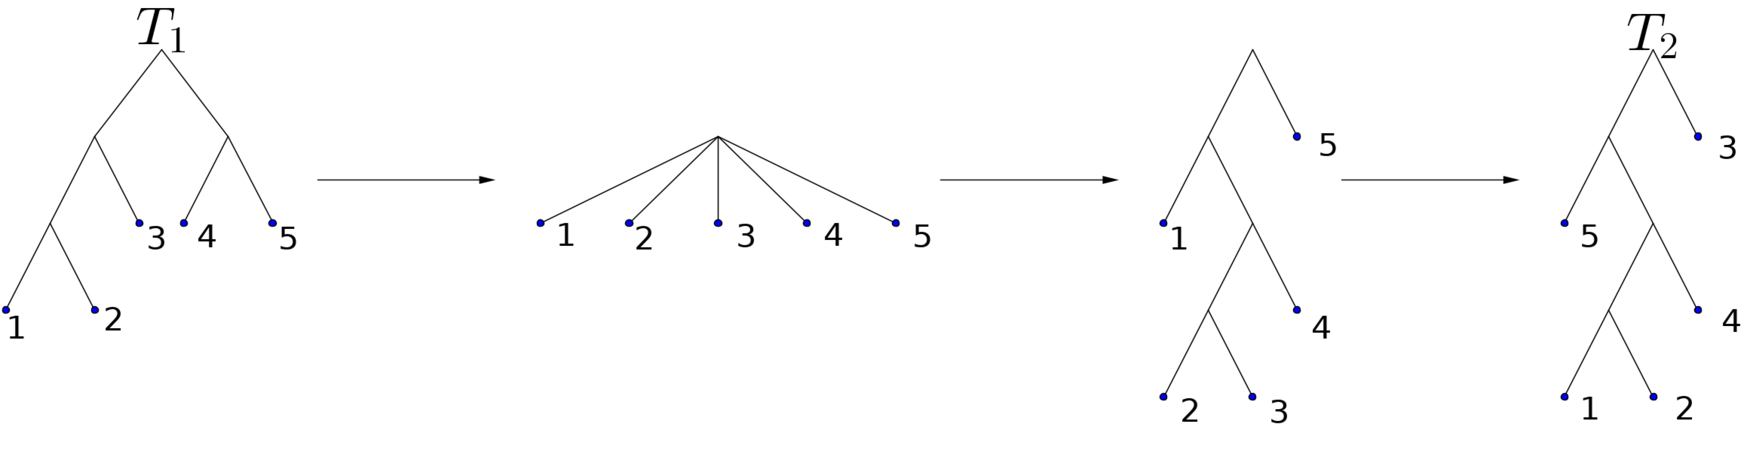
\includegraphics[width=0.90\textwidth]{figures/CTED.png}
		\caption{A step guide for limiting the CTED by the number of leaves.}
		\label{fig:CTED}
	\end{figure}
\end{proof}
\begin{rem}
	To calculate the actual average $\mathcal{A}_{CTED}(n)$ and whether it converges to $1$, one has to solve the following equation:
	$$\mathcal{A}_{CTED}(n) = (\sum_{i = 0}^n \, n - i \, \mathbb{P}(\pi \text{ has exactly $i$ fixpoints})) \frac{1}{n}$$
	where $\pi$ is an arbitrarily chosen permutation on the set $\{1,...,n\}$. 
\end{rem}
The second observation can be proven by the same procedure described in Lemma~\ref{lem:CTED}. The only difference is, that the first two steps both cost exactly $n-2$, as this is the number of interior nodes other than the root. 

These two observations only resemble the data found during the computations. There are many special cases, where the procedure from Lemma~\ref{lem:CTED} does not yield the best solution. For trees $T_1$ and $T_2$ in Figure~\ref{fig:maxRFdist} for example, the cheapest way to manipulate $T_1$ is to delete the leave with label $1$ and its parent, insert an interior node on the edge of the root to leave $8$ and append leaf $1$ as another child. Thus the overall costs of the manipulation are $2$. Nevertheless in most cases the observed costs resemble the costs of the above mentioned procedure. All these considerations are based on the fact, that the actual costs of the CTED only depend on the permutation of the leaves' labels, but not on the actual structure of the trees. Two completely differently structured trees may have a CTED distance of $0$ as long as the underlying permutation of the labels is the same one with respect to the left to right order. Thus the CTED can be seen as a distance measure on permutations, but it does not reflect useful information in the context of structured trees.\\
For the STED we saw that on the one hand, there are often better solutions than the plain procedure of deleting and inserting of all interior nodes, thus resembling more advanced solutions that indeed take the structure of the trees into account. On the other hand, this distance measure does not give a benefit on the interior nodes. Since we wanted to construct a distance measure that resembles the gRF while refining it, we failed to mainly concentrate on the clades and their leaves labels.

Last but not least, we calculated the values for the $\alpha$-ATED with different values for $\alpha$. It is obvious that the average $\mathcal{A}_{\alpha -ATED}(n)$ is directly proportional to $\alpha$. For $\alpha \to 0$ the average $\mathcal{A}_{\alpha -ATED}(n) \to \mathcal{A}_{CTED}(n)$, for $\alpha \to 1$ the average $\mathcal{A}_{\alpha -ATED}(n) \to \mathcal{A}_{STED}(n)$. Furthermore we can prove the upper bound on the average $\mathcal{A}_{\alpha -ATED}(n) < n +\frac{2n}{\alpha}$ by the same procedure as described in Lemma~\ref{lem:CTED}.
